\section{湍流预混火焰}
\subsection{概述}
\subsection{一些应用}
\subsubsection{电火花点火发动机}
\subsubsection{燃气轮机}
\subsubsection{工业气体燃烧器}
\subsection{湍流火焰传播速度定义}
\begin{equation}
    S_\mathrm{t} = \frac{\dot{m}}{\overline{A} \rho_u}
\end{equation}其中\(\dot{m}\)是反应物的质量流量;\(\rho_\mathrm{u}\)是未燃气体密度;\(\overline{A}\)是时间平滑后的火焰面积。这一速度也被称为\textbf{通用消耗速度}。
\subsection{湍流预混火焰结构}
\subsubsection{实验观察}
\begin{figure}[H]
    \centering
    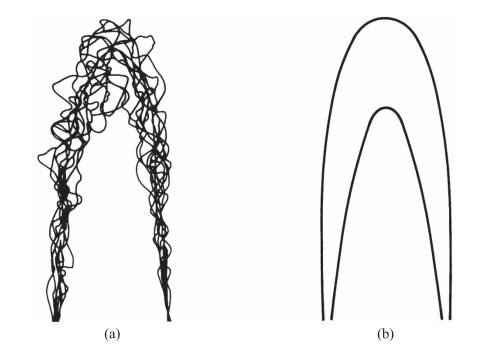
\includegraphics[width=.3\textwidth]{img/turb_prem_image.png}
\end{figure}
我们称这一有明显厚度的反应区为\textbf{湍流火焰刷}。瞬时的图像说明,实际的反应区像层流预混火焰一样,相对是很薄的。这些反应区有时也称为\textbf{层流火焰片}。

\subsubsection{三种火焰模式}

\begin{itemize}
    \item 褶皱层流火焰模式:\(\delta_L\le \mathcal{l}_\mathrm{K}\):威廉斯-克里莫夫(Williams-Klimov)判据。
    \item 分布反应模式:反应区内的输运现象就不仅受分子运动的控制,同时也受湍流运动的控制,或者至少要受湍流运动的影响。\(\delta_L > \mathcal{l}_0\):丹姆克尔(DamkGhler)判据。
    \item 漩涡小火焰模式:\(\mathcal{l}_0 > \delta_\mathrm{L} > \mathcal{l}_\mathrm{K}\)。
\end{itemize}

利用\(\mathcal{l}_\mathrm{K}\delta_\mathrm{L}\)和\(\mathcal{l}_0/\delta_\mathrm{L}\),湍流雷诺数\(Re_{t_0}\)和丹姆克尔数\(Da\),来进行分析。